
To judge the degradation of predictions of the algorithms with decreasing
information quality (detailed in Section \ref{sec:inforeduc2}), a plot for each
energy window list (auto, short, and long) is made.  Figure \ref{fig:rxtr}
shows the balanced accuracy of reactor type classification for the previously
described \textit{x}-axis, where a score of $1$ is perfect prediction and a
score of $0$ is random classification. The error bars reflect a 99\% confidence
interval. The red line that indicates a baseline/minimum acceptable performance
is at a balanced accuracy score of 0.84, which is based on the lowest
performance of all three algorithms at 20\% training set error for the 29
nuclide mass training set in Figure \ref{fig:randerrA}. The blue line that
indicates an ideal performance is at 0.97 balanced accuracy, which is based on
the approximate performance of all three algorithms at 5\% training set error
for the 29 nuclide mass training set. 

\begin{figure}[!htb]
  \centering
  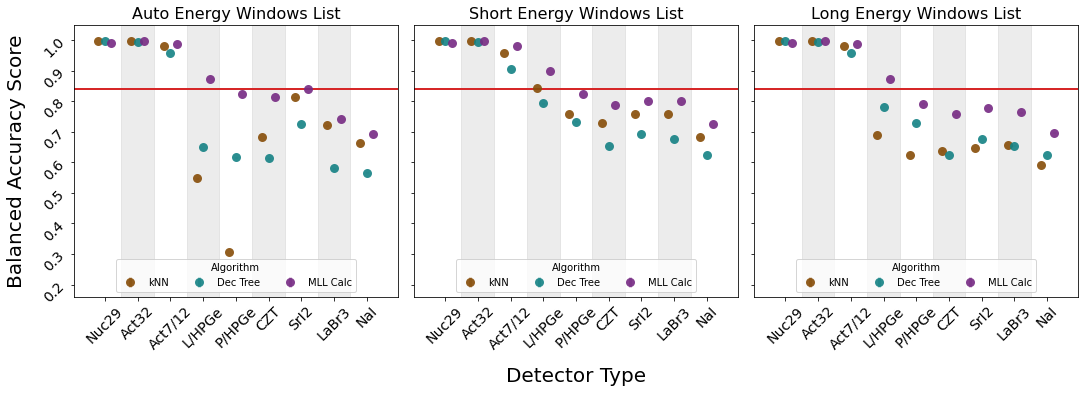
\includegraphics[width=\textwidth]{./chapters/exp2/detector_preds_wrt_enlist_BalAcc_rxtr.png}
  \caption{Prediction performance of reactor type as measured by balanced 
           accuracy with respect to decreasing detector energy resolution 
           for three types of processed gamma spectra.}
  \label{fig:rxtr}
\end{figure}

\begin{figure}[!htb]
  \centering
  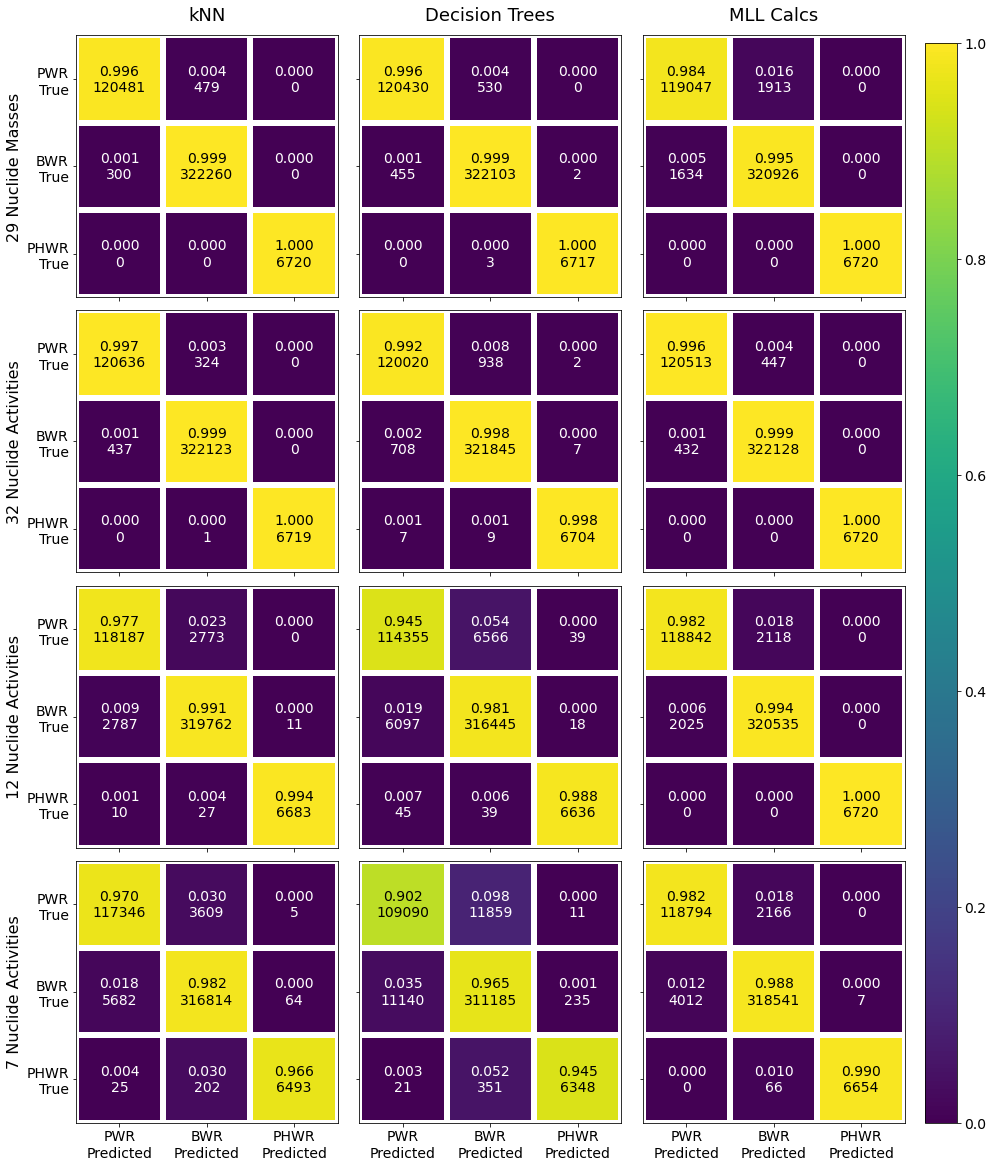
\includegraphics[width=\textwidth]{./chapters/exp2/confusion_matrix_nucs_acts.png}
  \caption{Confusion matrices of reactor type prediction for each algorithm 
           for different training sets (all at a 1\% error level): 29 nuclide 
           masses, 32 nuclide activities, 12 nuclide activities, and 7 nuclide 
           activities.}
  \label{fig:cm_nucs_acts}
\end{figure}

\begin{figure}[!htb]
  \centering
  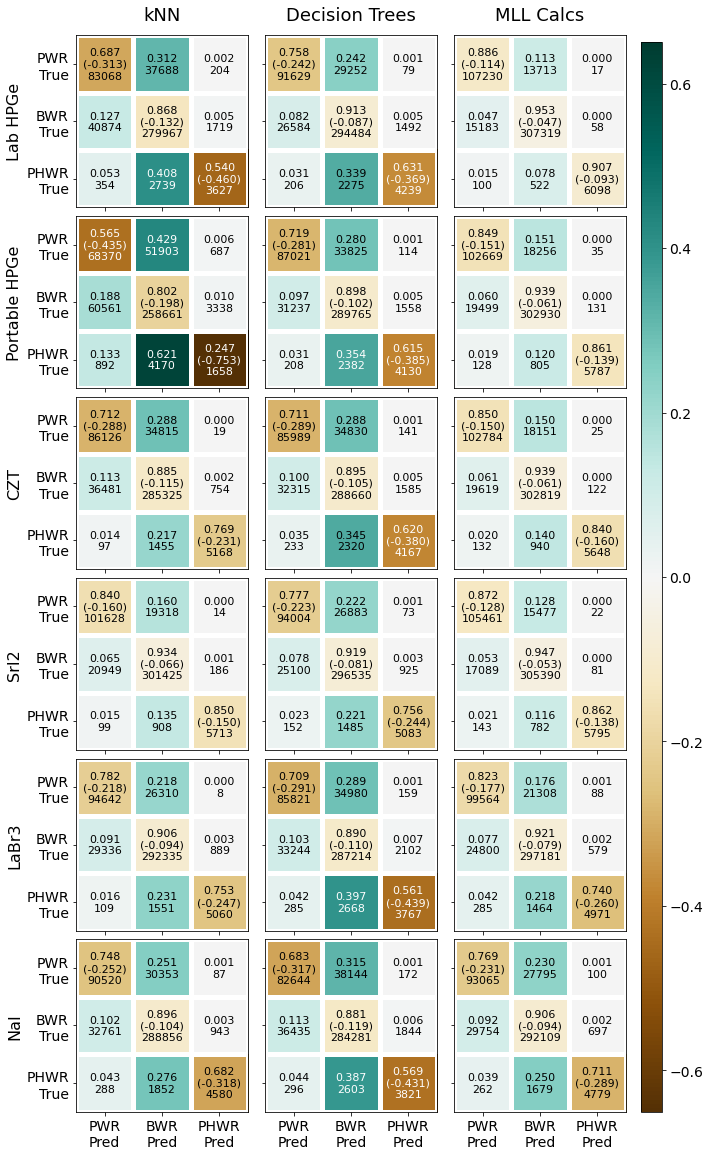
\includegraphics[width=0.83\textwidth]{./chapters/exp2/confusion_matrix_6dets_auto.png}
  \caption{Confusion matrices for auto energy window list training sets.}
  \label{fig:cm_auto}
\end{figure}

\begin{figure}[!htb]
  \centering
  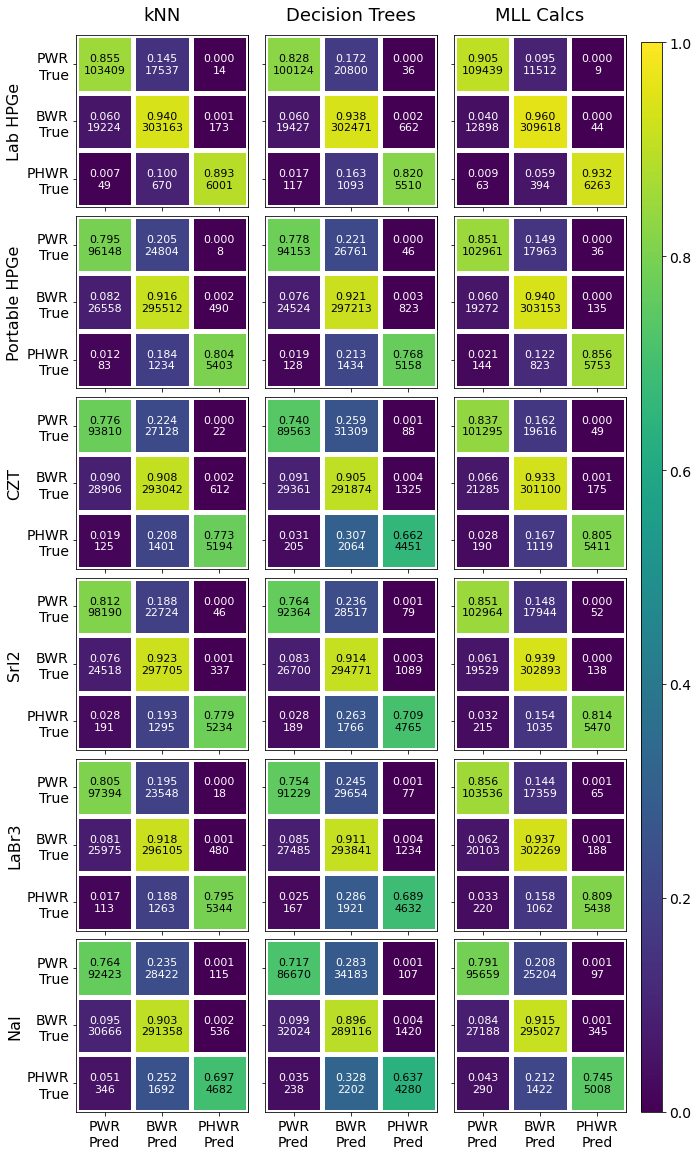
\includegraphics[width=0.83\textwidth]{./chapters/exp2/confusion_matrix_6dets_short.png}
  \caption{Confusion matrices for short energy window list training sets.}
  \label{fig:cm_short}
\end{figure}

\begin{figure}[!htb]
  \centering
  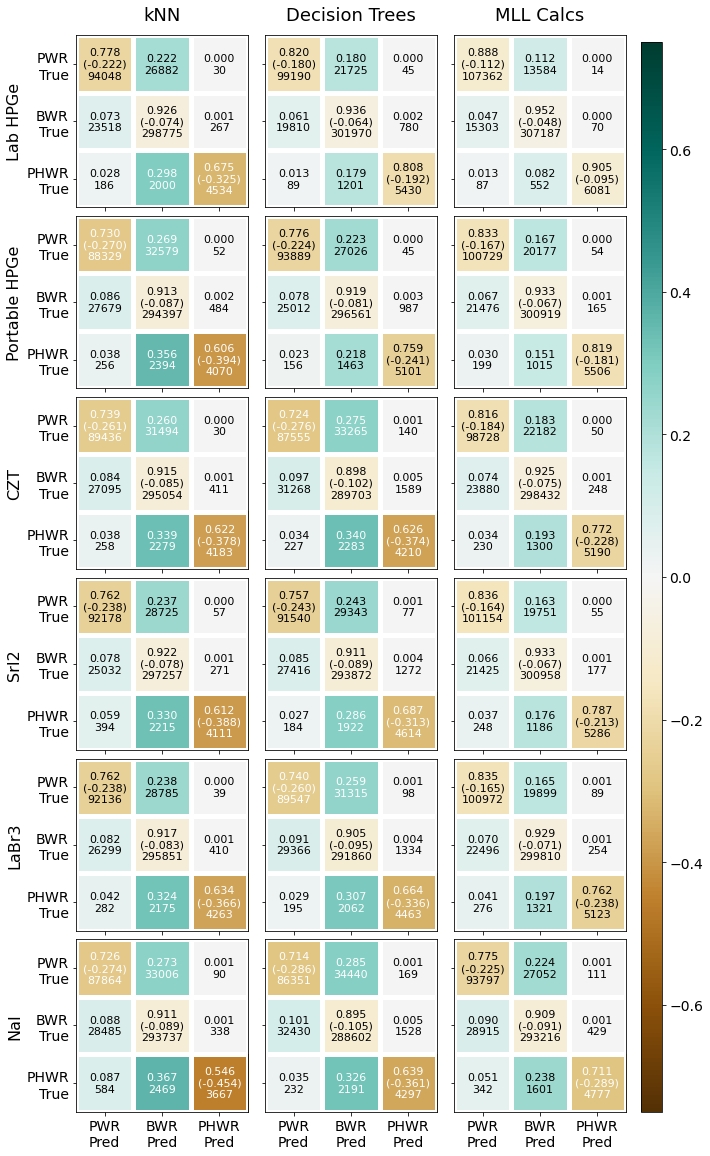
\includegraphics[width=0.83\textwidth]{./chapters/exp2/confusion_matrix_6dets_long.png}
  \caption{Confusion matrices for long energy window list training sets.}
  \label{fig:cm_long}
\end{figure}

